\documentclass{article}
\usepackage[english]{babel}
\usepackage[utf8]{inputenc}
\usepackage[margin=1.5cm]{geometry}
\usepackage{float}
\usepackage[sc]{mathpazo}
\title{COMP2208 Assignment: Search Methods \\“Blocksworld tile puzzle”}

\author{
  {\textbf{Alked Ejupi}}\\
  \\
  School of Electronics and Computer Science\\
  University of Southampton\\
  Student ID:   \texttt{30352118} \\
  \texttt{ae7g18@soton.ac.uk}
}
\date{November 2019}

\usepackage{dirtytalk}
\usepackage{natbib}
\usepackage{amsmath,amsthm,amssymb}
\usepackage{graphicx}

\usepackage{caption}
\usepackage{subcaption}

\def\code#1{\texttt{#1}}
\begin{document}

\maketitle

\vfil \break
\tableofcontents
\vfil \break

\section{Approach}
\subsection{Formulation of the blocks world puzzle}
Before the actual implementation of the search algorithms to solve the blocks world puzzle, a formal formulation of the \textbf{problem} is needed in order to achieve generalisation in terms of further scalability in the future. The first thing I have defined is the\textit{ \textbf{state} }of a board. This contains a description of the board in a particular time where it specifies the positions of each tile \textit{A}, \textit{B}, \textit{C} and the position of the Agent in a grid of size $NxN$ ($4x4$ in the case of the problem given). Once defined the structure of a single state, it was possible to formally describe the \textbf{initial state} describing the given initial configuration of the board. Another important aspect for defining the problem was specifying what were the \textbf{\textit{Actions}} of the agent that could be done on the board, this refers to the actions \textbf{\textit{UP}}, \textbf{\textit{DOWN}}, \textbf{\textit{LEFT}} and \textbf{\textit{RIGHT}}. In order to apply the move of an agent in a board, I have also defined the\textit{\textbf{ transition model}} where given a particular state and an action it returns a new state with the movement of the agent applied, obtaining a new configuration of the board. 

\subsection{Environment setup}

I choose \textit{Java} language to implement the blocks world and the search algorithms, as it is the language which I am most proficient with. I organised my Java project in way that I could easily add features without having the trouble to refactor the code or apply enormous changes to the existing code. The UML Diagram represented down below describes the structure of the projects. The \texttt{Utils.java} class contains methods that are used across the entire projects such as printing the state of the board in ASCII, common operations such as converting an array 2D to 1D or viceversa and..

\subsection{Defining the problem}
All the code related to the problem comes under the package named \code{Problem}. I decided to keep it as generic as possible, for this reason I defined an interface called \code{Problem.java} which includes all the information that the blocks world puzzle should have in order to be solved.

\begin{figure}[H]
\centering
\begin{subfigure}{.5\textwidth}
  \centering
  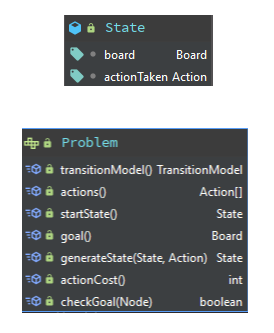
\includegraphics[width=.5\linewidth]{stateAndProblem.png}
  \label{fig:sub1}
\end{subfigure}%
\begin{subfigure}{.5\textwidth}
  \centering
  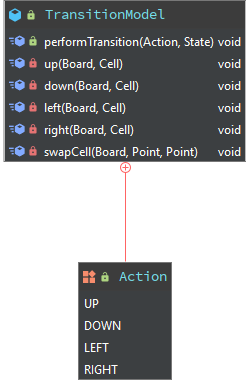
\includegraphics[width=.5\linewidth]{transition.png}
  \label{fig:sub2}
\end{subfigure}
\caption{\code{Problem} package}
\label{fig:test}
\end{figure}

\subsection{Implementing the blocks world}

All code related to the blocks world can be found under the package \texttt{BlocksWorld}. This includes the class \texttt{Cell} which defines a single cell of the board. The class \texttt{Board} describes the internal structure of a board, that is, a two dimensional array of cells (type \texttt{Cell}) . The \texttt{Cell} has also an inner enum class called \texttt{CellType} representing the types of cells in the blocks world, tile \textit{A}, \textit{B} and \textit{C}, \textit{Agent} and \textit{empty} cell. The board contains also a reference of each tile (A, B and C) and the Agent which are needed for finding their position.

\subsection{Tree Search implementation}
To help avoid code duplication I have created an abstract class called \texttt{TreeSearch.java}. This contains common operations and properties that search trees have, such as generating a child node and successors nodes, return a solution given a node, number of nodes, depth of the tree and the search method which refers to the strategy we want to use. The search method (\code{List<Node> search(Problem problem)}) is not implemented in \texttt{TreeSearch.java}, it is implemented in all search classes \texttt{BFS.java}, \texttt{DFS.java}, \texttt{IDS.java} and \texttt{AStar.java} according to the strategy they have. 
\par
 The class \code{Node.java} contains the attributes required to keep track of the tree we are constructing. These are the current \code{State}, the parent \code{Node}, the \code{Action} that was taken by the parent and the \code{pathCost} computed by summing all step cost from the initial state to the node.
 
 
 
 
 
 
 

\section{Evidence}
``I always thought something was fundamentally wrong with the universe'' \citep{adams1995hitchhiker}


\section{Scalability Study}


\section{Extras and limitations}
\section{Appendix}
\subsection{BFS}
\subsection{DFS}
\subsection{IDS}
\subsection{AStar}



\bibliographystyle{plain}
\bibliography{references}



\end{document}
